%
% IEEE Transactions on Microwave Theory and Techniques example
% Tibault Reveyrand - http://www.microwave.fr
%
% http://www.microwave.fr/LaTeX.html
% ---------------------------------------



% ================================================
% Please HIGHLIGHT the new inputs such like this :
% Text :
%  \hl{comment}
% Aligned Eq. 
% \begin{shaded}
% \end{shaded}
% ================================================



\documentclass[journal]{IEEEtran}

%\usepackage[retainorgcmds]{IEEEtrantools}
%\usepackage{bibentry}  
\usepackage{xcolor,soul,framed} %,caption

\colorlet{shadecolor}{yellow}
% \usepackage{color,soul}
\usepackage[pdftex]{graphicx}
\graphicspath{{../pdf/}{../jpeg/}}
\DeclareGraphicsExtensions{.pdf,.jpeg,.png}

\usepackage[cmex10]{amsmath}
%Mathabx do not work on ScribTex => Removed
%\usepackage{mathabx}
\usepackage{array}
\usepackage{mdwmath}
\usepackage{mdwtab}
\usepackage{eqparbox}
\usepackage{url}

%\bstctlcite{IEEE:BSTcontrol}


%=== TITLE & AUTHORS ====================================================================
\begin{document}
\title{Fast Network Threat Detection based on the TRAbID dataset: An Analysis of Various Machine Learning Models }
\author{
Shrey Agarwal,
Ashwini Hiremath,
Ibrahim Khalid,
Harsh Shinde,
Justin Wang%
\thanks{Dr. Shih Yu Chang}
}
% The paper headers
\markboth{Fast Network Threat Detection}{Fast Network Threat Detection}


\maketitle



\begin{abstract}
one sentence on problem, couple sentences on process, one or two sentences with the results
\end{abstract}

\begin{IEEEkeywords}
Network anomaly detection, Machine Learning
\end{IEEEkeywords}

\IEEEpeerreviewmaketitle

% === I. INTRODUCTION =============================================================
% =================================================================================
\section{Introduction}

\IEEEPARstart{I}{n} our ever increasing digital world, it is vital that we also have improved security over our networks. Based on the Cloudflare DDoS 2023 Q4 report \cite{cloudflare} and Verizon’s data breach report 2023 \cite{verizion}, there has been an increase in the number of cyber attacks, including network based attacks. By using live network data and classifying it as harmful or not, we can create a system that will improve the peace of mind of a user and allow them to use modern technology with confidence.

The primary objective of this project is to train various machine learning models for the classification of whether an activity on the network is a threat or not. The secondary objective of this project is to evaluate the machine learning models based on their performance, and computation time and cost in order to find the best model. This can be used to create a firewall application \cite{ucar2017analysis} that uses the built machine learning model.

\section{Proposed methodology}
We are planning to use the TRAbID dataset \cite{viegas2017toward} as it provides a relevant dataset for the problem, this can be subject to change. The TRAbID dataset is sufficiently large, with 44 feature columns, including classification, made up of generated network traffic data. Our methodology will be to first explore this dataset using tools such as Pandas, MatPlotLib, and Sci-Kit Learn. This includes tasks such as identifying correlations, normalizing values, and selecting important features. Following this, we will work on training a few different types of models in order to determine which models perform the best at distinguishing network threats. Models we plan on training are: Support Vector Machines, Logistic Regression, Naive Bayes, Random Forest, XGBoost, and K-Nearest Neighbors. These selected models can be subject to change. We will compare the models based on accuracy, precision and recall, and speed of classification.

\section{Literature review}
Bagui et al. \cite{bagui2019using} explored the UNSW-NB15 dataset \cite{moustafa2015unsw} using a hybrid approach that used k-means clustering followed by decision trees or Naive Bayes. Bhati et al. \cite{bhati2022ensemble} used the KDDCUP99 dataset to explore the effectiveness of ensemble models such as AdaBoost and Random Forest. Viegas et al. \cite{viegas2017toward} generated the TRAbID dataset with the goal of providing a better dataset for training machine learning models. They trained on this dataset using the Naive Bayes and Decision Tree algorithms. Based on our short literature review among the listed papers and otherwise, there has not been a clear strive for creating a model with the goal of fast detection after training. We plan on furthering research in this regard by exploring the effectiveness of various machine learning techniques on the TRAbID dataset.

\section{Hypothesis}
The anticipated results include improved organizational knowledge and awareness of the cyber threat landscape, allowing for improved readiness and response tactics. Furthermore, by adding to the body of knowledge on cybersecurity, these assessments hope to enhance defense systems and policies. The expected outcome of this research is to find a model that is able to quickly and accurately classify network traffic data. Future work based use cases on this research project would be to create a live network monitoring firewall application that can quickly run network traffic through a trained model and notify the user in case of a network based attack.

\section{Data Process}

\section{Exploratory Data Analysis}

\section{Modelling}
\subsection{Designing benchmark}
\subsection{model 1}
\subsection{model 2}
\subsection{model 3}
\subsection{model 4}
\subsection{model 5}

\section{Results and comparison}

\section{Conclusion}

% \begin{figure}[!htb]
%   \centering
%   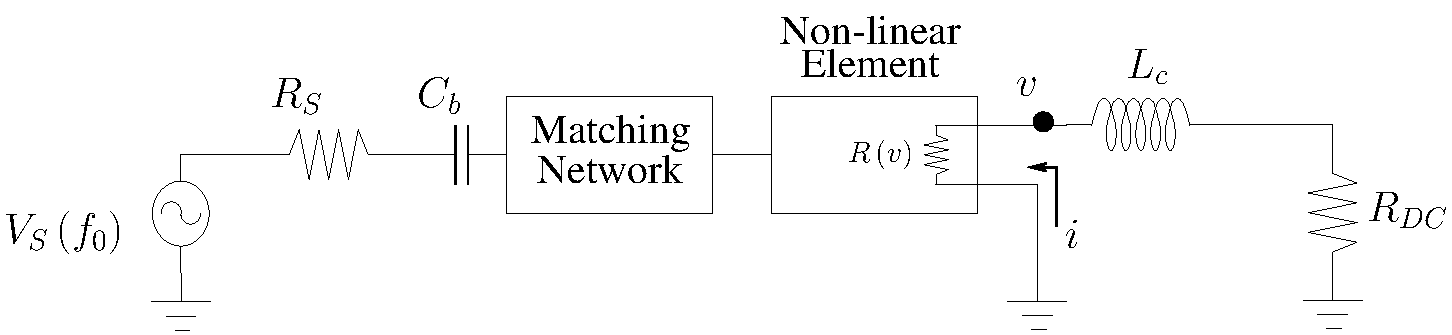
\includegraphics[width=\linewidth]{figures/01.pdf}
%   \caption{This is how to add a figure and caption}
%   \label{circuit_diagram}
% \end{figure}

% This is how to reference a Fig.~\ref{circuit_diagram}.

% This is how to write an equation and reference it like eq. \ref{ideal_rectifier_resistance}.
% \begin{equation}
% \label{ideal_rectifier_resistance}
% R(v) =
% \begin{cases}
%     \infty, & v > 0\\
%     0, & v \leq 0
% \end{cases}
% \end{equation}

% \begin{itemize}
%     \item This
%     \item is
%     \item how to make an unnumbered list
% \end{itemize}


% \begin{enumerate}
%     \item This
%     \item is
%     \item how to make a numbered list
% \end{enumerate}

\ifCLASSOPTIONcaptionsoff
  \newpage
\fi

\bibliographystyle{IEEEtran}
\bibliography{IEEEabrv,Bibliography}

% \begin{IEEEbiography}[{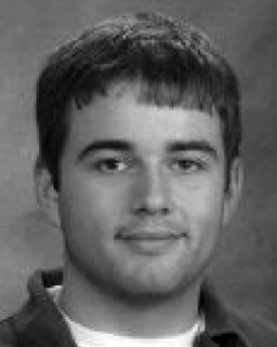
\includegraphics[width=1in,height=1.25in,clip,keepaspectratio]{photo/mike.png}}]{Michael Roberg}
% Do we need a bio section? We should ask the professor
% \end{IEEEbiography}
\vfill
\end{document}